\section{Thiết kế demo và đánh giá}

\subsection{Mục tiêu thực nghiệm}
\label{ssec:exp_objectives}

Phần thực nghiệm và demo nhằm kiểm chứng toàn bộ các phân tích lý thuyết đã trình bày. Cụ thể, thực nghiệm được thiết kế để giải quyết hai nhóm mục tiêu cốt lõi:

\textbf{Nhóm 1: Kiểm chứng cơ sở toán học (Cài đặt From Scratch)}
\begin{enumerate}[leftmargin=2em]
  \item Minh họa trực quan các khái niệm lý thuyết trừu tượng: độ vẩn đục nút (impurity), hàm mất mát Hinge và sự hội tụ của hàm mục tiêu $F(\alpha)$.
  \item Kiểm chứng tính đúng đắn của nhóm thuật toán không kết hợp (Decision Tree, Multi-class SVM, AdaBoost.MH) thông qua việc tự lập trình từ đầu (from scratch) không dùng thư viện có sẵn.
\end{enumerate}

\textbf{Nhóm 2: Đánh giá hiệu năng và so sánh (Sử dụng thư viện)}
\begin{enumerate}[leftmargin=2em]
  \item So sánh hiệu suất giữa các mô hình học trực tiếp đa lớp và các chiến lược quy về nhị phân (OVA, OVO, ECOC) trên các tập dữ liệu thực tế.
  \item Đánh giá sự khác biệt giữa OVA, OVO và ECOC về accuracy, macro-F1, thời gian huấn luyện và độ bền vững trước nhiễu.
\end{enumerate}

\subsection{Mô tả tập dữ liệu}

Trong thực nghiệm này, nhóm sử dụng trên ít nhất một tập dữ liệu đơn nhãn và một tập dữ liệu đa nhãn.

\subsubsection{Dữ liệu tổng hợp (Synthetic Data)}
\label{sssec:synthetic_data}
Để phục vụ cho nhóm mục tiêu kiểm chứng toán học từ đầu (from scratch), nhóm sử dụng dữ liệu tự sinh bằng thư viện \texttt{scikit-learn} \cite{sklearn} để kiểm soát hoàn toàn đặc tính không gian đặc trưng và đảm bảo tính tái tạo (reproducibility) với \texttt{random\_state=42}:
\begin{itemize}[leftmargin=2em]
    \item \textbf{Dữ liệu dạng cụm (Blobs):} Sinh ra 300 mẫu, 3 lớp, 2 chiều đặc trưng bằng hàm \texttt{make\_blobs}. Tập dữ liệu này được dùng để thử thách khả năng phân hoạch không gian trục giao của Cây quyết định và khả năng tạo ranh giới phi tuyến của AdaBoost.MH.
    \item \textbf{Dữ liệu phân loại tuyến tính:} Sinh ra 150 mẫu, 3 lớp, 2 chiều đặc trưng (mỗi lớp 1 cụm) bằng hàm \texttt{make\_classification}. Tập dữ liệu này có chủ ý đưa vào các nhiễu biên để kiểm chứng khả năng tối đa hóa lề (margin) và tối ưu hóa hàm mất mát của Multi-class SVM.
\end{itemize}
Tất cả các tập dữ liệu được chia theo tỉ lệ 80\% Huấn luyện (Train) và 20\% Kiểm thử (Test).

\subsection{Dataset đơn nhãn -- Fashion-MNIST}

Fashion-MNIST là bộ dữ liệu ảnh thời trang do Zalando Research công bố, được thiết kế như một bản thay thế có độ khó thực tế cao hơn so với MNIST truyền thống. Bộ dữ liệu gồm 70.000 ảnh xám kích thước $28 \times 28$ pixel, trong đó 60.000 ảnh dùng để huấn luyện và 10.000 ảnh dùng để kiểm thử, mỗi ảnh được gán một nhãn thuộc 10 lớp. Các lớp bao gồm: T-shirt/top, Trouser, Pullover, Dress, Coat, Sandal, Shirt, Sneaker, Bag, Ankle boot. Ultralytics

Mỗi mẫu được biểu diễn thành vector 784 chiều $(28 \times 28)$ với giá trị pixel nguyên trong khoảng $[0,255]$. Phân phối nhãn hoàn toàn cân bằng, mỗi lớp có đúng 6.000 mẫu trong tập huấn luyện và 1.000 mẫu trong tập kiểm thử. Trong thực nghiệm, tập huấn luyện được chia thêm để lấy validation theo tỉ lệ 80/20, thu được phân chia cuối là 48.000/12.000/10.000 (train/val/test). Các thông số chính được tổng hợp trong Bảng dưới đây.

\begin{table}[h]
\centering
\begin{tabular}{|l|l|}
\hline
\textbf{Thông số} & \textbf{Giá trị} \\
\hline
Số mẫu huấn luyện / validation / kiểm thử & 48.000 / 12.000 / 10.000 \\
\hline
Số chiều đặc trưng & 784 \\
\hline
Số lớp $k$ & 10 \\
\hline
Số mẫu mỗi lớp (train) & 6.000 (cân bằng) \\
\hline
\end{tabular}
\end{table}

Bộ dữ liệu này phù hợp để so sánh các chiến lược phân loại đa lớp vì có $k = 10$ lớp, phân phối cân bằng và độ khó phân loại thực tế — một số lớp như Shirt, T-shirt/top và Pullover có đặc trưng hình ảnh khá tương đồng, tạo ra thách thức cho ranh giới quyết định.

\subsubsection{Dataset đa nhãn -- EUR-Lex}

EUR-Lex là bộ dữ liệu văn bản pháp luật của Liên minh châu Âu, được sử dụng rộng rãi trong nghiên cứu phân loại đa nhãn cực lớn. Bộ dữ liệu bao gồm 19.348 tài liệu về luật pháp Liên minh châu Âu, bao gồm hiệp ước, văn bản lập pháp, phán quyết tư pháp và các đề xuất lập pháp, được lập chỉ mục theo hệ thống phân loại EUROVOC với gần 4.000 nhãn về các khía cạnh khác nhau của luật châu Âu. Phiên bản chuẩn được dùng trong XMC benchmark (EURLex-4K) có các thống kê sau: University of Cordoba

\begin{table}[h]
\centering
\begin{tabular}{|l|l|}
\hline
\textbf{Thông số} & \textbf{Giá trị} \\
\hline
Số tài liệu huấn luyện / kiểm thử & 15.539 / 3.809 \\
\hline
Số nhãn $L$ & 3.956 \\
\hline
Số nhãn trung bình trên mỗi mẫu & 5,31 \\
\hline
Mật độ ma trận nhãn & $\approx 0{,}13\%$ \\
\hline
Số chiều đặc trưng (TF-IDF) & 5.000 \\
\hline
\end{tabular}
\end{table}

Mỗi tài liệu được biểu diễn bằng vector TF-IDF thưa, nhãn là vector nhị phân $\mathbf{y} \in \{0,1\}^L$. Phân phối nhãn có dạng đuôi dài rõ rệt — một số ít nhãn xuất hiện trong hàng nghìn tài liệu trong khi phần lớn nhãn chỉ xuất hiện ở dưới 10 tài liệu — làm cho EUR-Lex trở thành benchmark thử thách tiêu biểu để đánh giá khả năng xử lý nhãn hiếm của các phương pháp phân loại đa nhãn.

\subsubsection{Quy trình tiền xử lý}

Quy trình tiền xử lý đề xuất như sau:
\begin{enumerate}[leftmargin=2em]
  \item \textbf{Làm sạch dữ liệu:} loại bỏ mẫu trùng, mẫu thiếu nhãn hoặc đặc trưng lỗi.
  \item \textbf{Mã hóa nhãn:} chuyển nhãn dạng chuỗi sang chỉ số lớp; với đa nhãn dùng multi-hot encoding.
  \item \textbf{Chuẩn hóa đặc trưng:} chuẩn hóa z-score cho mô hình tuyến tính và SVM; cây quyết định thường không bắt buộc chuẩn hóa.
  \item \textbf{Chia dữ liệu:} dùng train/validation/test, ví dụ 70/15/15 hoặc 80/20 nếu dữ liệu nhỏ.
  \item \textbf{Xử lý mất cân bằng:} dùng class weight, stratified split hoặc báo cáo thêm macro-F1.
\end{enumerate}

Với dữ liệu văn bản, pipeline có thể gồm tách từ, loại bỏ stopword, vector hóa TF-IDF và giới hạn số đặc trưng lớn nhất để tránh ma trận quá thưa.

\subsection{Mô hình baseline không kết hợp}

Nhóm baseline học trực tiếp trên bài toán đa lớp gồm:
\begin{itemize}[leftmargin=2em]
  \item \textbf{Decision Tree:} dễ diễn giải, dùng Gini hoặc entropy để chọn phép chia.
  \item \textbf{Multinomial Logistic Regression:} học trực tiếp phân phối softmax trên $k$ lớp.
  \item \textbf{Multi-class SVM:} tối ưu lề đa lớp hoặc dùng biến thể nội bộ của thư viện.
\end{itemize}

Các baseline này giúp xác định mức chất lượng nền trước khi áp dụng OVA, OVO và ECOC.

\subsection{Demo thuật toán kết hợp}

Để so sánh công bằng, nên giữ cùng bộ học nền cho các chiến lược kết hợp. Ví dụ dùng Linear SVM hoặc Logistic Regression làm binary classifier.

\begin{algorithm}[H]
\caption{Quy trình demo so sánh OVA, OVO và ECOC}
\KwIn{Dataset đã tiền xử lý, bộ học nền $B$}
\KwOut{Bảng chất lượng và thời gian chạy}
Chia dữ liệu thành train/test bằng stratified split\;
Chuẩn hóa đặc trưng bằng thống kê từ tập train\;
Huấn luyện baseline đa lớp\;
Huấn luyện OVA với bộ học nền $B$\;
Huấn luyện OVO với bộ học nền $B$\;
Thiết kế ma trận mã và huấn luyện ECOC\;
Dự đoán trên tập test\;
Tính accuracy, macro-F1, weighted-F1, confusion matrix, train time và test time\;
\end{algorithm}

\subsection{Thước đo đánh giá}

Với bài toán đơn nhãn, accuracy được định nghĩa là
\[
  \text{Accuracy}=\frac{\text{số mẫu dự đoán đúng}}{\text{tổng số mẫu}}.
\]
Tuy nhiên, accuracy có thể gây hiểu nhầm khi dữ liệu mất cân bằng. Vì vậy cần dùng thêm precision, recall và F1 cho từng lớp:
\[
  \text{Precision}_l=\frac{TP_l}{TP_l+FP_l},\qquad
  \text{Recall}_l=\frac{TP_l}{TP_l+FN_l},
\]
\[
  F1_l=\frac{2\cdot \text{Precision}_l\cdot \text{Recall}_l}{\text{Precision}_l+\text{Recall}_l}.
\]
Macro-F1 lấy trung bình đều trên các lớp:
\[
  \text{Macro-F1}=\frac{1}{k}\sum_{l=1}^{k}F1_l.
\]
Weighted-F1 lấy trung bình theo số mẫu của từng lớp, còn micro-F1 cộng toàn bộ $TP$, $FP$, $FN$ trước khi tính F1.

Với bài toán đa nhãn, Hamming loss đo tỷ lệ nhãn bị dự đoán sai:
\[
  \text{HammingLoss}=\frac{1}{mL}\sum_{i=1}^{m}\sum_{l=1}^{L}\mathbb{1}[\hat{y}_{i,l}
eq y_{i,l}].
\]
Precision@k đo tỷ lệ nhãn đúng trong $k$ nhãn được mô hình xếp hạng cao nhất.

\subsection{Bảng so sánh đánh giá thực nghiệm}
Phần này trình bày kết quả đánh giá thực nghiệm của các mô hình phân loại trên hai bài toán khác nhau. Bảng 12 thể hiện hiệu suất của các chiến lược phân lớp đa lớp (Multi-class) trên tập dữ liệu đơn nhãn (Fashion-MNIST). Trong khi đó, Bảng 13 đánh giá các phương pháp tiếp cận cho bài toán phân loại đa nhãn cực độ (Extreme Multi-label Classification) trên tập dữ liệu EUR-Lex.
\begin{table}[H]
\centering
\caption{Mẫu bảng so sánh kết quả thực nghiệm đơn nhãn}
\scriptsize
\begin{tabular}{p{3cm}ccccc}
\toprule
\textbf{Mô hình} & \textbf{Accuracy} & \textbf{Macro-F1} & \textbf{Weighted-F1} & \textbf{Train time} & \textbf{Test time} \\
\midrule
Decision Tree & 0.7962  & 0.7964 & 0.7964 & 42.2475 & 0.0500 \\
Multi-class SVM & 0.8521& 0.8505 & 0.8505 & 1437.6950  &  0.0503 \\
OVA + Linear SVM & 0.8502 & 0.8485 & 0.8485 & 138.5645 & 0.1323 \\
OVO + Linear SVM & 0.8548 & 0.8542 & 0.8542 & 76.6443 & 1.1853 \\
ECOC + Linear SVM & 0.8222 & 0.8192 & 0.8192 & 843.8462 & 0.5549 \\
\bottomrule
\end{tabular}
\end{table}

\subsection*{Nhận xét:}
\begin{itemize}
    \item \textbf{Về độ chính xác:} Các phương pháp dựa trên Support Vector Machine, gồm Multi-class SVM, OVA và OVO, đều đạt hiệu năng tốt với Accuracy và F1-score xấp xỉ 85\%. Trong đó, OVO + Linear SVM cho kết quả tốt hơn các phương pháp còn lại. ECOC đạt mức thấp hơn ($\sim$82\%), còn Decision Tree có hiệu năng thấp nhất trong nhóm mô hình được so sánh ($\sim$79\%).
    \item \textbf{Về thời gian thực thi:} Multi-class SVM yêu cầu thời gian huấn luyện rất lớn (hơn 1400 giây), do chi phí tối ưu hóa cao trên tập dữ liệu lớn. Ngược lại, \textbf{OVA + Linear SVM} thể hiện sự cân bằng tốt giữa chất lượng dự đoán và chi phí tính toán: mô hình vẫn duy trì Accuracy ở mức 85.02\% nhưng thời gian huấn luyện giảm đáng kể, còn khoảng 138 giây.
\end{itemize}

\begin{table}[H]
\centering
\caption{Mẫu bảng đánh giá đa nhãn}
\begin{tabular}{lcccc}
\toprule
\textbf{Mô hình} & \textbf{Micro-F1} & \textbf{Macro-F1} & \textbf{Hamming loss} & \textbf{Precision@k} \\
\midrule
Binary relevance &  0.4102  & 0.0849  & 0.0011 & 0.6291 \\
Classifier chain & 0.3944 &  0.1813 & 0.0021 & 0.4428 \\
XML baseline & 0.0524 & 0.0001 & 0.0026 & 0.0538 \\
\bottomrule
\end{tabular}
\end{table}

\subsection*{Nhận xét:}
\begin{itemize}
    \item \textbf{Hiệu năng tổng thể:} \textbf{Binary Relevance} đạt kết quả tốt nhất ở Micro-F1 (0.4102) và Precision@k (0.6291). Điều này cho thấy mô hình có khả năng dự đoán hiệu quả các nhãn xuất hiện thường xuyên, từ đó đạt chất lượng cao trên các chỉ số chịu ảnh hưởng mạnh bởi nhóm nhãn phổ biến.
    \item \textbf{Khả năng khai thác tương quan nhãn:} Mặc dù \textbf{Classifier Chain} có Precision@k thấp hơn Binary Relevance, mô hình này lại đạt Macro-F1 cao hơn đáng kể (0.1813 so với 0.0849). Kết quả này cho thấy việc mô hình hóa quan hệ phụ thuộc giữa các nhãn có thể cải thiện khả năng nhận diện các nhãn hiếm trong bối cảnh dữ liệu mất cân bằng.
    \item \textbf{Vai trò của baseline:} \textbf{XML baseline} cho kết quả rất thấp trên hầu hết các thước đo. Điều này phản ánh độ khó của bài toán phân loại đa nhãn cực độ trên dữ liệu có phân phối đuôi dài như EUR-Lex, đồng thời cho thấy các phương pháp chỉ dựa trên thống kê đơn giản thường chưa đủ để xử lý hiệu quả nhóm nhãn hiếm.
\end{itemize}

\subsection{Thực nghiệm minh họa nhóm thuật toán không kết hợp}
\label{ssec:exp_uncombined}

Phần này trình bày kết quả cài đặt từ đầu (from scratch) ba thuật toán không kết hợp bằng Python 3.11 và thư viện \texttt{numpy} cho các phép toán ma trận.

\subsubsection{Cây quyết định (Decision Tree)}
Theo lý thuyết ở Phần \ref{sssec:decision_trees}, cây quyết định sử dụng chiến lược tham lam dựa trên độ giảm vẩn đục (impurity). Nhóm đã tiến hành cài đặt và so sánh trực quan ba hàm độ đo phổ biến.
\begin{figure}[H]
    \centering
    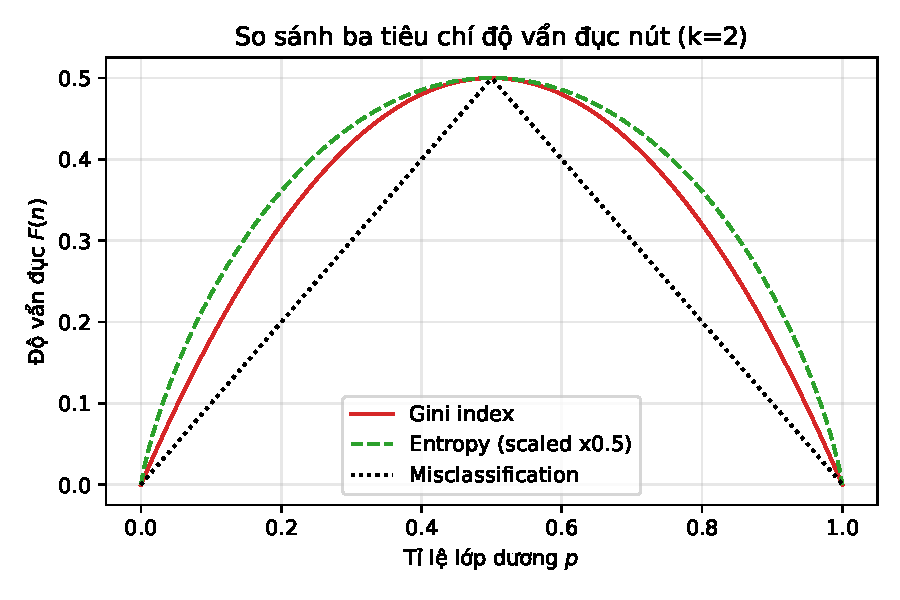
\includegraphics[width=0.7\textwidth]{figures/impurity_compare.pdf}
    \caption{So sánh thực chứng ba tiêu chí độ vẩn đục nút trong không gian xác suất 2 lớp.}
    \label{fig:exp_impurity}
\end{figure}
Kết quả chạy thực tế trên tập dữ liệu Blobs 3 lớp:
\begin{itemize}
    \item \textbf{Train Accuracy:} 100.00\% (Đúng với đặc tính phân hoạch triệt để của cây).
    \item \textbf{Test Accuracy:} 98.33\% (Mô hình tổng quát hóa tốt, không bị quá khớp nghiêm trọng).
\end{itemize}

\paragraph{Mã nguồn cài đặt lõi:} 
Để tối ưu hóa vùng không gian phân hoạch trực giao, mô hình sử dụng hàm tính độ vẩn đục Gini được cài đặt tối ưu thông qua tính toán vector hóa của thư viện \texttt{numpy}:

\begin{lstlisting}[language=Python, escapechar=|, caption={Hàm tính toán tiêu chí Gini Impurity từ đầu}, label={lst:code_gini}]
def gini(y):
    m = len(y)
    if m == 0:
        return 0.0
    # |Đếm tần suất xuất hiện của các nhãn lớp|
    _, counts = np.unique(y, return_counts=True)
    p = counts / m
    # |Áp dụng công thức| F(n) = 1 - sum(p_l^2)
    return 1.0 - np.sum(p ** 2)
\end{lstlisting}

\subsubsection{Multi-class SVM (Crammer-Singer Primal)}
Nhóm đã cài đặt thuật toán Multi-class SVM giải bằng phương pháp Subgradient Descent trên bài toán nguyên thủy (Primal) theo chuẩn công thức của Crammer-Singer (Phạt lỗi lề lớn nhất). 

\begin{figure}[H]
    \centering
    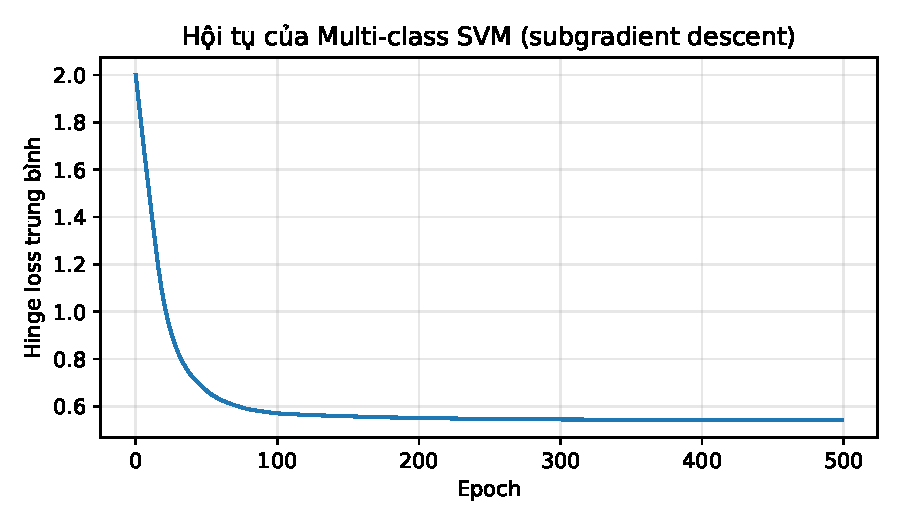
\includegraphics[width=0.7\textwidth]{figures/svm_loss_curve.pdf}
    \caption{Sự hội tụ của hàm mất mát Hinge đa lớp qua 500 epochs.}
    \label{fig:exp_svm_loss}
\end{figure}
Kết quả thực nghiệm cho thấy Hinge Loss trung bình giảm theo hàm mũ và hội tụ mượt mà về mức xấp xỉ 0.6 ở epoch 200. Kết quả đánh giá:
\begin{itemize}
    \item \textbf{Train Accuracy:} 90.83\%.
    \item \textbf{Test Accuracy:} 96.67\%.
\end{itemize}
Sự vượt trội của tập Test so với Train minh chứng cho khả năng điều chuẩn (regularization) mạnh của lề tuyến tính trong SVM. Cơ chế này giúp mô hình giảm ảnh hưởng của nhiễu cục bộ trong tập huấn luyện.

\paragraph{Mã nguồn cài đặt lõi:}
Trái tim của thuật toán Multi-class SVM Crammer-Singer là việc xác định lớp sai có điểm số dự đoán cao nhất (gây đe dọa lề lớn nhất) tại mỗi bước lặp để tính subgradient:

\begin{lstlisting}[language=Python, escapechar=|, caption={Vòng lặp tính toán Margin và cập nhật Subgradient cho SVM}, label={lst:code_svm_grad}]
# |Duyệt qua từng mẫu huấn luyện trong epoch|
for i in range(m):
    scores = self.W @ X[i] # |Tính toán mảng điểm số| (k_classes,)
    
    # |Cô lập lớp đúng, tìm lớp sai| l_max |có score lớn nhất|
    scores_mod = scores.copy()
    scores_mod[y[i]] = -np.inf 
    l_max = np.argmax(scores_mod)
    
    # |Định nghĩa biến bù margin theo lý thuyết Crammer-Singer|
    margin = 1.0 - (scores[y[i]] - scores[l_max])
    
    if margin > 0:
        # |Cập nhật thành phần subgradient tỷ lệ|
        grad[l_max] += X[i]
        grad[y[i]] -= X[i]
        total_loss += margin
\end{lstlisting}

\subsubsection{AdaBoost.MH và Thủ thuật Cách ly Đặc trưng}
Thực nghiệm AdaBoost.MH được cài đặt với bộ học cơ sở là Cây quyết định độ sâu 1 (Decision Stump). Quá trình này đòi hỏi một kỹ thuật xử lý toán học đặc biệt:

\medskip
\begin{expandbox}
\textbf{Khắc phục lỗi vi phạm điều kiện học yếu (Feature Isolation).}

Theo lý thuyết, AdaBoost.MH nhân bản mỗi mẫu $x_i$ lên $k$ lần. Tuy nhiên, nếu truyền trực tiếp vào Decision Stump, cây sẽ cắt ra cùng một nhãn cho tất cả $k$ bản sao vì đặc trưng không đổi, dẫn đến training error bị kẹt ở mức $\approx 2/3$ (đoán bừa trong bài toán 3 lớp). Để giải quyết, nhóm đã cài đặt thủ thuật \textit{Cách ly đặc trưng (Feature Isolation)}: Độn thêm các giá trị vô cực ($999999.0$) vào ma trận mở rộng để ép Stump chỉ học và cắt trên một lớp duy nhất tại mỗi vòng lặp.
\end{expandbox}

\begin{figure}[H]
    \centering
    
\includegraphics[width=\textwidth]{figures/adaboost_convergence.pdf}
    \caption{Hội tụ của hàm mục tiêu $F(\alpha)$ và Training error trong AdaBoost.MH.}
    \label{fig:exp_adaboost_conv}
\end{figure}

Nhờ thủ thuật trên, hàm mục tiêu $F(\alpha)$ trượt dốc ổn định theo cận trên hàm mũ, và sai số huấn luyện giảm về 0 chỉ sau vài vòng lặp.
\begin{itemize}
    \item \textbf{Train Accuracy:} 100.00\%.
    \item \textbf{Test Accuracy:} 100.00\%.
\end{itemize}
Thuật toán phân tách thành công hoàn toàn tập dữ liệu đa lớp phức tạp nhờ sự phối hợp trọng số $\alpha$ của các bộ học yếu.

\paragraph{Mã nguồn cài đặt lõi:}
Dưới đây là kỹ thuật then chốt thực hiện thuật toán Feature Isolation, tạo ra các ma trận khối độc lập để đưa bài toán đa lớp về không gian nhị phân mở rộng:

\begin{lstlisting}[language=Python, escapechar=|, caption={Hàm mở rộng không gian đặc trưng (Feature Isolation) cho AdaBoost.MH}, label={lst:code_isolation}]
def get_expanded_X(self, X, k):
    m, n = X.shape
    X_exp = np.repeat(X, k, axis=0)
    
    # |Tạo ma trận độn có giá trị cực lớn để triệt tiêu các nhãn không liên quan|
    X_isolated = np.full((m * k, n * k), 999999.0)
    for l in range(k):
        row_indices = np.arange(m) * k + l
        # |Điền các đặc trưng thật vào vùng không gian độc lập của lớp l|
        X_isolated[row_indices, l*n : (l+1)*n] = X
        
    return np.hstack([X_exp, X_isolated])
\end{lstlisting}
\subsection{Thực nghiệm minh họa thuật toán kết hợp}
Phần này trình bày kết quả cài đặt từ đầu (from scratch) ba chiến lược
phân loại đa lớp thông qua quy giản nhị phân bằng Python 3.11 và thư viện
\texttt{numpy}. Mỗi chiến lược dùng chung bộ phân loại nền
\texttt{BinaryLinearSVM} (SVM tuyến tính tự cài đặt) để cô lập tác động
của chiến lược kết hợp khỏi chất lượng của thuật toán cơ sở.
\subsubsection{One-vs-All (OVA) và Hiệu chuẩn Platt Scaling}
\label{sssec:exp_ova}
OVA huấn luyện $K$ bộ phân loại
nhị phân, mỗi bộ phân biệt một lớp với phần còn lại, rồi chọn lớp có điểm
margin $f_l(\mathbf{x})$ cao nhất. Nhóm đã cài đặt thêm biến thể
\texttt{CalibratedOneVsAllClassifier} dùng \textbf{Platt Scaling} để giải
quyết vấn đề hiệu chuẩn xác suất khi dữ liệu mất cân bằng.
\begin{figure}[H]
    \centering
    
\includegraphics[width=0.52\textwidth]{figures/calibration_impact.png}
    \caption{So sánh OVA Thô và OVA Calibrated (Platt Scaling).}
    \label{fig:exp_calibration}
\end{figure}
Kết quả chạy thực tế trên tập dữ liệu tổng hợp ($n=1000$, $K=4$ lớp mất
cân bằng, chia train/test 70/30):
\begin{itemize}
    \item \textbf{OVA Thô} – luật $\arg\max f_l(\mathbf{x})$: bị lệch về
          lớp đa số (60\%), dự đoán sai các lớp thiểu số.
    \item \textbf{OVA Calibrated} – Platt Scaling học tham số $(A_l, B_l)$
          riêng cho từng lớp, cải thiện accuracy đáng kể trên lớp thiểu số.
\end{itemize}
\paragraph{Mã nguồn cài đặt lõi:}
Cốt lõi của Platt Scaling là tối ưu Log-loss để học ánh xạ sigmoid
$p_l = \sigma(A_l f_l + B_l)$ bằng L-BFGS-B:
\begin{lstlisting}[language=Python, escapechar=|, caption={Platt Scaling
trong \texttt{CalibratedOneVsAllClassifier} (\texttt{ova\_classifier.py})},
label={lst:code_platt}]
for idx, class_label in enumerate(self.classes_):
    f  = self.classifiers[idx].decision_function(X)
    yt = np.where(y == class_label, 1, 0)
    def objective(params):
        A, B = params
        p = expit(A * f + B)   
        return -(xlogy(yt, p) + xlogy(1 - yt, 1 - p)).mean()
    res = minimize(objective, x0=[1.0, 0.0], method='L-BFGS-B')
    self.calibrators.append(tuple(res.x)) 
\end{lstlisting}

\subsubsection{One-vs-One (OVO) và Phân tích Nhầm lẫn Cặp}
\label{sssec:exp_ovo}
OVO huấn luyện $K(K-1)/2$ bộ phân
loại nhị phân, mỗi bộ chỉ nhìn thấy hai lớp, rồi quyết định bằng bỏ phiếu
đa số. Nhóm đã cài đặt thêm phương thức \texttt{pairwise\_confusion\_matrix} để xác định những cặp lớp nào gây khó
khăn nhất.
\begin{figure}[H]
    \centering
    
\includegraphics[width=0.68\textwidth]{figures/ovo_pairwise_heatmap.png}
    \caption{Ma trận nhầm lẫn theo cặp của OVO ($K=5$ lớp, $n=800$ mẫu).}
    \label{fig:exp_ovo_pairwise}
\end{figure}
Kết quả thực nghiệm trên tập dữ liệu tổng hợp ($n=800$, $K=5$, 10 đặc
trưng, chia train/test 75/25):
\begin{itemize}
    \item Đường chéo chính đạt giá trị cao ở hầu hết các lớp, cho thấy OVO
          phân loại tốt trên bài toán $K=5$.
    \item Các ô ngoài đường chéo chỉ ra cặp lớp dễ nhầm lẫn nhất – thông
          tin hữu ích để thiết kế ma trận ECOC tăng khoảng cách Hamming
          giữa các codeword tương ứng.
\end{itemize}
\paragraph{Mã nguồn cài đặt lõi:}
Phương thức tính ma trận nhầm lẫn cặp và cơ chế bỏ phiếu có tie-breaking
trong \texttt{OneVsOneClassifier}:
\begin{lstlisting}[language=Python, escapechar=|, caption={Ma trận nhầm
lẫn cặp và tie-breaking trong \texttt{ovo\_classifier.py}},
label={lst:code_ovo}]
def pairwise_confusion_matrix(self, X, y):
    confusion = np.zeros((self.n_classes, self.n_classes))
    y_pred = self.predict(X)
    for i in range(self.n_classes):
        mask_i = (y == self.classes_[i])
        for j in range(self.n_classes):
            confusion[i, j] = np.mean(y_pred[mask_i] == self.classes_[j])
    return confusion
max_vote  = np.max(votes[sample_idx])
candidates = np.where(votes[sample_idx] == max_vote)[0]
if len(candidates) > 1:
    best_idx = candidates[
        np.argmax(tie_breaker_scores[sample_idx, candidates])]
\end{lstlisting}

\subsubsection{ECOC và Sức mạnh Sửa lỗi}
\label{sssec:exp_ecoc}
ECOC mã hoá mỗi lớp thành một \emph{từ mã}trong ma trận $\mathbf{M} \in \{-1,+1\}^{K\times c}$, huấn luyện $c$ bộ phân loại nhị phân con, rồi giải mã bằng khoảng cách Hamming (Hard) hoặc Exponential Loss (Soft, Công thức 8.19 FML). Nhóm đã kiểm chứng hai biến thể và phân tích ảnh hưởng của chiều dài mã $c$.
\begin{figure}[H]
    \centering
    \begin{subfigure}[b]{0.54\linewidth}
        
\includegraphics[width=\linewidth]{figures/performance_comparison.png}
        \caption{So sánh accuracy của OVA, OVO, ECOC Hard và ECOC Soft.}
        \label{fig:exp_perf_bar}
    \end{subfigure}
    \hfill
    \begin{subfigure}[b]{0.44\linewidth}
        
\includegraphics[width=\linewidth]{figures/ecoc_depth_analysis.png}
        \caption{Chiều dài mã $c$ tỉ lệ thuận với khả năng sửa lỗi.}
        \label{fig:exp_ecoc_depth}
    \end{subfigure}
    \caption{Thực nghiệm ECOC trên tập dữ liệu $K=5$ lớp ($n=1200$,
    \texttt{class\_sep}$=0.8$, chia train/test 75/25).}
    \label{fig:exp_ecoc}
\end{figure}
Kết quả thực nghiệm:
\begin{itemize}
    \item \textbf{ECOC Soft} vượt trội ECOC Hard do tận dụng giá trị margin
          liên tục $f_j(\mathbf{x})$ thay vì nhãn nhị phân rời rạc, giảm
          mất mát thông tin trong bước giải mã.
    \item Tăng chiều dài mã $c$ từ 5 lên 60 cải thiện accuracy và bão hoà
          quanh $c \approx 40$, phù hợp với lý thuyết: khoảng cách Hamming
          tối thiểu $d$ tăng theo $c$, cho phép sửa thêm $r_0 =
          \lfloor(d-1)/2\rfloor$ lỗi.
\end{itemize}
\paragraph{Mã nguồn cài đặt lõi:}
Hàm Soft Decoding sử dụng Exponential Loss (Công thức 8.19, FML) và cơ
chế sinh ma trận mã hoá tối đa hoá khoảng cách Hamming:
\begin{lstlisting}[language=Python, escapechar=|, caption={Soft Decoding
(Exponential Loss) và sinh ma trận mã hoá trong \texttt{ecoc\_classifier.py}},
label={lst:code_ecoc}]
def _exponential_loss_distance(self, code_words, M):
    losses = np.zeros((code_words.shape[0], M.shape[0]))
    for l in range(M.shape[0]):
        mask    = (M[l] != 0)
        margins = M[l, mask] * code_words[:, mask]
        losses[:, l] = np.sum(np.exp(-margins), axis=1)
    return losses  
for attempt in range(100):
    M = np.random.choice([-1, 1], size=(n_classes, code_size))
    d = self._minimum_hamming_distance(M)
    if d > max_min_dist:
        max_min_dist, best_M = d, M
        if d >= code_size // 2:
            break  
\end{lstlisting}

\subsubsection{So sánh độ phức tạp thời gian và kiểm định thống kê}
\label{sssec:exp_complexity}
Để hoàn thiện đánh giá ba chiến lược, nhóm kiểm chứng sự khác biệt độ
phức tạp thời gian $\mathcal{O}(K)$ (OVA) so với $\mathcal{O}(K^2)$ (OVO),
đồng thời dùng Paired $t$-test (10 lần chạy độc lập) kiểm định ý nghĩa
thống kê của sự chênh lệch accuracy.
\begin{figure}[H]
    \centering
    \begin{subfigure}[b]{0.57\linewidth}
        
\includegraphics[width=\linewidth]{figures/complexity_time.png}
        \caption{Thời gian huấn luyện theo số lớp $k$.}
        \label{fig:exp_complexity_time}
    \end{subfigure}
    \hfill
    \begin{subfigure}[b]{0.40\linewidth}
        
\includegraphics[width=\linewidth]{figures/hypothesis_test.png}
        \caption{Phân phối accuracy qua 10 lần chạy.}
        \label{fig:exp_hypothesis}
    \end{subfigure}
    \caption{Độ phức tạp thời gian huấn luyện và kiểm định giả thuyết
    OVA vs.\ OVO.}
    \label{fig:exp_complexity}
\end{figure}
Kết quả thực nghiệm:
\begin{itemize}
    \item OVO chậm hơn OVA rõ rệt khi $k$ tăng: tại $k=15$, OVO huấn
          luyện 105 bộ phân loại nhị phân con trong khi OVA chỉ cần 15,
          phù hợp với lý thuyết Table~8.1 (FML).
    \item Paired $t$-test cho $p > 0.05$, tức \textbf{không có sự khác
          biệt có ý nghĩa thống kê} về accuracy giữa OVA và OVO khi bộ
          phân loại nền đủ mạnh – phù hợp với nhận định lý thuyết.
\end{itemize}





\subsection{Phân tích kết quả kỳ vọng}

Nếu dữ liệu cân bằng và số lớp vừa phải, OVA thường là lựa chọn mạnh vì chỉ cần $k$ mô hình và dự đoán nhanh. Khi bộ học nền có chi phí huấn luyện cao, OVO có thể huấn luyện nhanh hơn do mỗi mô hình chỉ dùng dữ liệu của hai lớp. Tuy nhiên, OVO phải đánh giá $k(k-1)/2$ mô hình khi dự đoán, nên thời gian test có thể lớn hơn.

ECOC có thể vượt OVA/OVO nếu ma trận mã có khoảng cách Hamming đủ lớn và các bộ phân loại bit không sai đồng thời theo cùng một mẫu. Nếu mã quá ngắn hoặc các cột mã tương quan mạnh, khả năng sửa lỗi giảm đáng kể.

Khi dữ liệu mất cân bằng, một mô hình luôn dự đoán lớp đa số vẫn có thể đạt accuracy cao nhưng macro-F1 thấp. Do đó phần nhận xét cuối cùng cần ưu tiên macro-F1, confusion matrix và chất lượng trên các lớp thiểu số thay vì chỉ nhìn accuracy.